% !TeX root = ../index.tex
\documentclass[../index.tex]{subfiles}

\begin{document}
    \section{Wykład 4}
        \subsection{Klasa jasności}
            Widma tego samego typu mogą mieć różnej szerokości linie widmowe. Szerokość linii zależy od ciśnienia panującego w fotosferach gwiazd. Im większe ciśnienie tym większe rozmycie linii widmowych. Te różnice w rozmyciach linii widmowych spowodowały wprowadzenia drugiego parametru w klasyfikacji widmowej \--- \textbf{klasy jasności}. Najważniejszych klas jasności jest 8, są one oznaczane kolejnymi liczbami rzymskimi i posiadają swoje nazwy:
            \begin{itemize}
                \item Hiperolbrzym (0).
                \item Nadolbrzym (I).
                \item Jasny olbrzym (II).
                \item Olbrzym (III).
                \item Podolbrzym (IV).
                \item Karzeł = gwiazda ciągu głównego (V).
                \item Podkarzeł (VI).
                \item Biały karzeł (VII).
            \end{itemize}
            Najczęściej spotykanymi klasami jasności są karły (szczególnie zimne czerwone karły). Pełna \textbf{klasyfikacja widmowa słońca to G2V}.
        \subsection{Diagram Hertzsprunga-Russella}
            Pierwotnie był to diagram, który na osi OX umieszczony miał typ widmowy od O do M, a na osi OY jasność absolutną (klasę jasności). Później pojawiły się inne warianty, w których zamiast typu widmowego umieszczony jest wskaźnik barwy albo logarytm \(T_\text{eff}\), a substytutem jasności absolutnej logarytm moc promieniowania gwiazdy \(L\). Poniżej przedstawione są dwa warianty tego wykresu. Na lewym diagramie ciągłe linie tyczą się jednej klasy jasności, a ich przebieg określa średnie położenie gwiazd danego typu. W górnej części diagramu grupują się hiperolbrzymy i nadolbrzymy. Na przekątnej występują karły, tzw. gwiazdy \textbf{ciągu głównego}. Od ciągu głównego odbiega \textbf{gałąź olbrzymów}. Na prawym wykresie widać głównie gwiazdy ciągu głównego i gałąź olbrzymów. Jak widać nie wszystkie kombinacje temperatury efektywnej i mocy promieniowania są możliwe.
            \begin{center}
                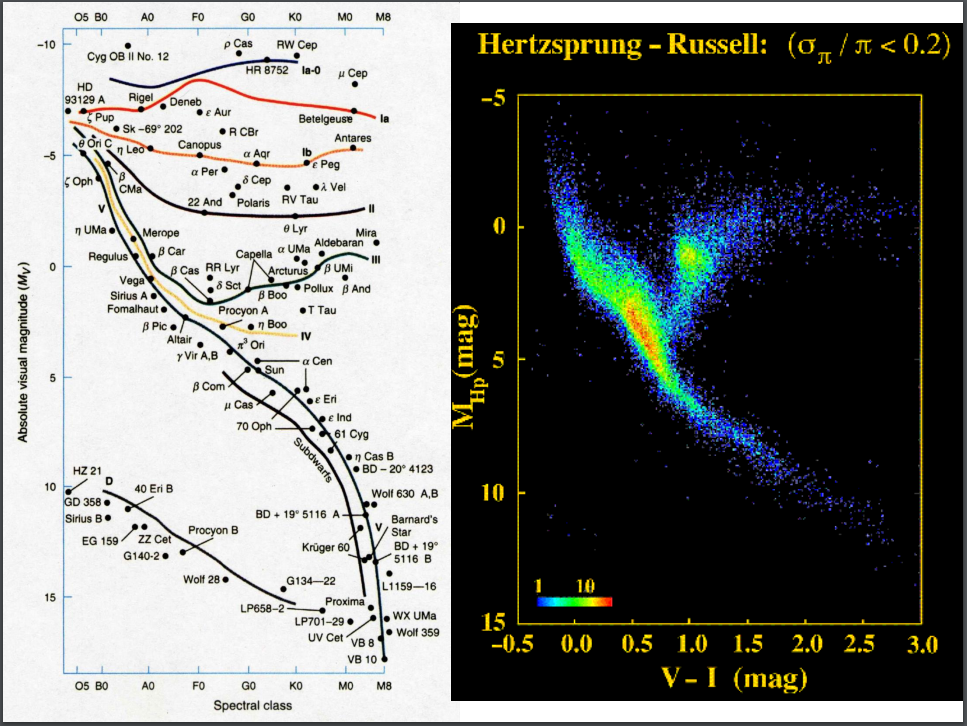
\includegraphics[width=16cm]{images/Hertzsprung-Russell.png}
            \end{center}
            Główną zaletą diagramu H-R jest możliwość wnioskowania na podstawie położenia gwiazdy o jej innych, nieznanych bezpośrednio parametrach.\\
            Korzystając z zależności:
            \begin{equation}
                L = 4\pi R^2 \sigma T_\text{eff}^{4}
            \end{equation}
            można nanieść na wykres linie jednakowego promienia i zauważyć, że największe gwiazdy znajdują się w prawym górnym rogu, a najmniejsze w lewym dolnym:
            \begin{center}
                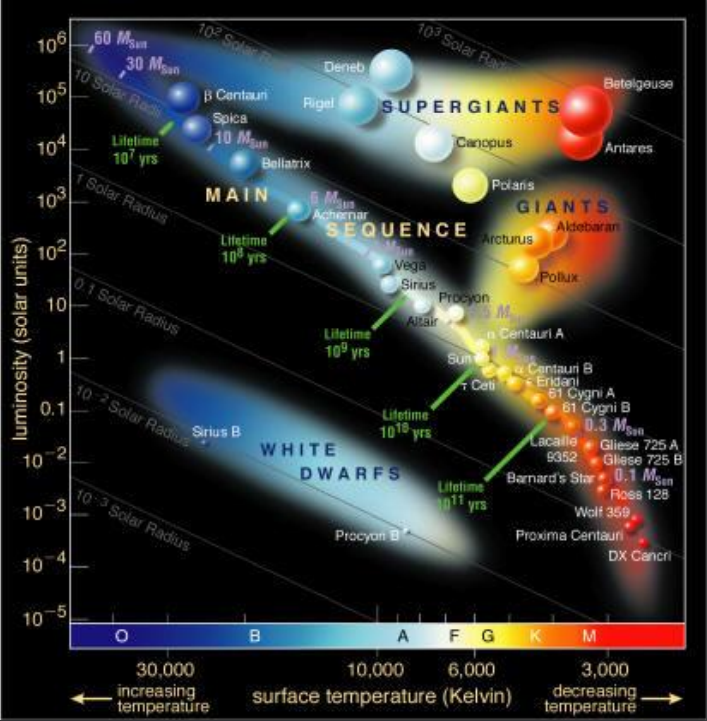
\includegraphics[width=10cm]{images/Hertzsprung-Russell-2.png}
            \end{center}
            Ścisłe przypisanie każdej klasy jasności do jakiegoś fragmentu diagramu H-R pozwala na skorzystanie ze wzoru \ref{eq:absolute_magnitudo}:
            \begin{equation}
                m - M = 5 \log D[pc] - 5 \tag{\ref{eq:absolute_magnitudo}}
            \end{equation}
            w celu określenia odległości. Wyznaczona w ten sposób odległość nazywana sie \textbf{paralaksą spektralną}.\\
            Położenie na diagramie konkretnej gwiazdy nie jest stałe. Gwiazdy w trakcie swojego życia ewoluują zmieniając swoje parametry i klasę jasności.
        \subsection{Masa gwiazdowa}
            Masa jest najważniejszym parametrem charakteryzującym gwiazdę. Najłatwiej jest ją ocenić obserwując skutki jej oddziaływania grawitacyjnego. W tym kontekście najwięcej oferują układy podwójne gwiazd. Ze względu na to w jaki sposób dowiadujemy się, że mamy do czynienia z układem podwójnym dzielimy je na \textbf{wizualne}, \textbf{spektroskopowe} i \textbf{zaćmieniowe}. 
            \subsubsection{Układy wizualne} 
                W procesie mierzenia masy układów podwójnych korzysta się z \textbf{uogólnionego III prawa Keplera}:
                \begin{equation}
                    \frac{P^2}{a^3 }(M_A + M_B) = \frac{4\pi^2}{G}
                \end{equation}
                gdzie \(P\) to okres obiegu, \(a\) to długość dłuższej półosi elipsy, a \(G\) stała grawitacji. Przyrównując w ten sposób układ ziemia-słońce z układem podwójnym otrzymuje się wzór:
                \begin{equation}
                    \frac{P^2}{a^3 }(M_A + M_B) = \frac{P_0^2}{a_0^3 }(M_S + M_Z) 
                \end{equation}
                a z tego:
                \begin{equation}
                    (M_A + M_B)[M_S] = \frac{a^3[AU]}{P^2[\text{lata ziemskie}]}  
                \end{equation}
                Obserwując jedynie ruch względny w układzie można zebrać pomiary sumy mas gwiazd. Żeby otrzymać informacje o ich stosunku należy zmierzyć ruch względem środka masy i skorzystać ze wzoru:
                \begin{equation}
                    m_A r_A = m_B r_B
                \end{equation}
                W tego typu trudno zmierzyć układy podwójne o okresach krótszych niż rok i dłuższych niż 1000 lat. Te pierwsze ze względu na bardzo małe odległości między nimi (nie da się ich odróżnić nawet najlepszymi teleskopami), a tu drugie ze względu na bardzo powolny ruch względny.\\
                Ważną cechą układów wizualnie podwójnych jest to, że można je umieścić w przestrzeni trójwymiarowej, mimo tego, że obserwujemy jedynie rzut na płaszczyznę nieba (oszczędzę tutaj tej konstrukcji).
            \subsubsection{Uklady spektroskopowe}
                Tutaj o układzie dowiadujemy się na podstawie okresowych zmian w widmie związanych \textbf{przesunięciami dopplerowskich}. Skupiając się na widmach można zaobserwować cykliczną zmianę długości fali linii widma. Znając \(\lambda_0\) tzn. laboratoryjna długość fali danej linii widmowej można określić radialną składową ruchu gwiazdy w układzie podwójnym ze wzoru:
                \begin{equation}
                    \frac{v_r}{c}  = \frac{\lambda -\lambda_0}{\lambda_0} 
                \end{equation} 
                Zmiana wartości \(v_r(t)\) w czasie określa \textit{ruchliwość} gwiazdy i jest dobrym substytutem odległości od środka masy układu. Zdolność pomiaru takiego efektu jest jednak ograniczona \--- dla okresów dłuższych niż kilkanaście lat ruch wewnątrz układu jest tak niewielki, że przesunięcia dopplerowskie przestają być widoczne.\\
                Korzystając z tej metody można obserwować układy o bardzo krótkich okresach nawet krótszych niż doba ziemska. W przypadku takich można zaobserwować głównie orbity o ekscentryczności równej 0 (tzn. idealne okręgi). Uważa się to za dowód intensywnego oddziaływania grawitacyjnego pomiędzy gwiazdami w układzie.
            \subsubsection{Układy zaćmieniowe}
                W tym przypadku można zaobserwować cykliczne spadki jasności. Znajdujemy się niemal dokładnie w płaszczyźnie orbity gwiazd tworzących ten układ. Kiedy słabiej świecąca gwiazda zakrywa tę jaśniejszą mamy \textbf{zaćmienie główne}, a gdy odwrotnie \textbf{zaćmienie wtórnym}. Dzięki analizie zmian jasności można także dowiedzieć się o składnikach tworzących taki układ, np. określić rozmiar, kształt każdej z gwiazd oraz szczegóły rozkładu jasności na ich powierzchniach. Dalsza analiza pozwala też określić kąt \(i\) \--- kąt między płaszczyzną ukłądu, a płaszczyzną ekliptyki.
            \subsubsection{Gwiazdy ciągu głównego}
                Dla gwiazd ciągu głównego spełniona jest zależność masa-jasność. To znaczy, że dla każdej takiej gwiazdy możemy określić jej masę na podstawie przynależność określonego podtypu widmowego (lokalizacji na wykresie HR).
            \subsubsection{Pozostałe informacje o masie}
                Dolny zakres możliwych mas gwiazd to \(0.08 M_S\) \--- to dolna granica dla której może zachodzić fuzja jądrowa. Obiekty mniej masywne nazywamy \textbf{brązowymi karłami}. Górny zakres możliwych mas jest trudniejszy do zdefiniowania ze względu n
\end{document}